% Sommerville  - System architecture
% Sommerville  - System requirements specification
% Sommerville  - System models
% Sommerville  - Appendices
% Smith  - Requirements  - Specific System Description  - Problem Description  - Physical System Description
% Smith  - Requirements  - Specific System Description  - Solution Characteristics Specification
% Hewitt  - Application Design  - Design patterns
% Smith  - Design Specification
% Hewitt  - Application Design  - Scalability and performance
% Hewitt  - Application Design  - Extensibility
% Smith  - Requirements  - Likely Changes
% all of Hewitt  - Data Design
% Smith  - Requirements  - Requirements  - Nonfunctional Requirements
% sections 1 and 2 of Hewitt  - Infrastructure Design

\newsectionnobreak{Design specification}{sec:DDF_spec}
Template given. Describe modules and hierarchy of modules. Also describes likely and unlikely changes to the code.
Anticipated changes guide the design: ideally a change affects only one module

%How to decompose into modules?

The design specification may need to be supplemented by a Module Interface Specification (MIS).
More concrete in defining access routines and syntax, but still abstract in not defining how
things are done.

Use of VECMA/SEAVEA as framework
UQ by ensembles,  active subspaces (from \cite{y3re242}) and GPs for surrogates (from \cite{y3re252}).

%For an example of write once, re-use many times, see the \F{smardda-misc}
%software~\cite{miscwebsite}, which is Fortran-based and illustrates the concept.
The proposed \nep\ development is of sufficient complexity that the production
of code should be as automatic as as possible, and the `write once, use many times'
principle implies that the starting point for code generation will often be \LaTeX \ or Markdown format
documents from the DJF or indeed DDF.

For \nep, the initial write should be in  \LaTeX \ format representing an extension
of the tabular layout used to generate \Tab{symbols}, for conversion to \F{Doxygen} input
format for documentation and C++ source, specifying:
\begin{itemize}
\item variable name, which for \nep \ should be generated from \LaTeX \ using
substitutions set out in \Tab{twoclatex}.
\item brief description, to remind user what is the purpose of the variable
\item units
\begin{itemize}
\item physical units should be SI, except eV for temperatures and mm for CAD inputs
\item scale factors for extreme-valued fields, eg.\ $10^{18}$  for number densities, 
or for quantised fields, eg.\ position expressed in units of separation of a uniform grid.
\end{itemize}
\item default value(s) on input
\item simple constraints on variable values
\begin{itemize}
\item whether real number or integer-valued
\item range specification, eg.\ $0 <  n \leq 10$ if $n$ must be a positive, small integer
\end{itemize}
\item detailed description of what variable does, if not covered by group description.
\item constraints in terms of other variables
\end{itemize}
Input variables are grouped according to the objects/classes which they help define.

\F{smardda-misc} illustrates how to produce software that auto-generates the equivalent
of .h files to describe objects and and .cpp or .m  files for 
\begin{enumerate}
\item setting default values of variables
\item dumping inputs to .log text-files if required
\item checking constraints on input variables
\item saving acceptable values 
\end{enumerate}

\clearpage
\newsection{Objects/classes}{sec:DDF_objects}
\textbf{Notes} Procedures denoted in boldface, as separate sections.\\
\emph{n-D} does not include time\\
\cite{sciplan} in exc.bib

\subsection{Base classes}\label{sec:base-classes}
The proposed base classes for \nep\ are listed below and shown graphically in \Fig{baseclasses}.
\begin{figure}
\centerline{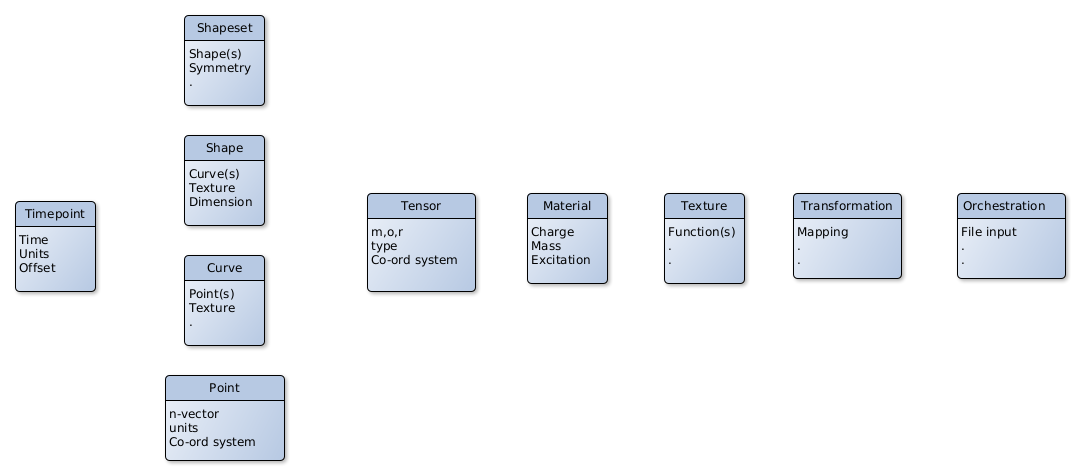
\includegraphics[width=0.7\textwidth]{./pics/baseclasses.png}}
\caption{\nep \ base classes.
\label{fig:baseclasses}}
\end{figure}

\begin{itemize}
\item
  Timepoint : point in physical time Attributes of time, units, offset
  (Alternatively just real scalar)
\item
  Point : point in \emph{n-D} space\\
  many make curve, shape;\\
  is particle location in \emph{n-D} ; Attributes of n-vector, units,
  coordinate system (Alternatively just real n-vector)
\item
  Curve : parts are one or more points, straight lines or textures
  or from CAD input or CSG input;\\
  many make shape;\\
  is shape boundary, is particle trajectory, is ray
\item
  Shape : parts are curves and textures, planar rectangles, or
  surfaces from CAD input or CSG input;\\
  many make Shapeset;\\
  is surface which aggregates as BC
\item
  Shapeset : parts are shapes, regular lattice, or volumes from CAD
  input or CSG input;\\
  is finite element geometry, is unstructured mesh, is surface geometry
  of body, is volume in \emph{n-D}, $n\geq 3$ ;\\
  helps defines field\\
  Attributes of degree of toroidal symmetry
\item
  Tensor : parts are $m$ numbers at a point, order $o$, type eg.\ 
  \emph{udd}, and density $r$ in \emph{n-D} coordinate system of type
  \emph{c};\\
  is ($m=3$, $o=1$, $n=3$) velocity, is ($m=1$, $o=3$,
  $n=3$) density,\\
  is ($m=1$, $o=0$, $n=3$) temperature, is ($m=3$, $o=0$,
  $n=0$) is array;\\
  many help make field (\emph{u} denotes contravariant, \emph{d} denotes
  covariant, \emph{c} defines cartesian, cylindrical, toroidal
  coordinates, $r=0$ usually)
\item
  Material : from database input ;\\
  helps make body, particle, many make matexture, plasma\\
  Attributes of charge, excitation level and mass
\item
  Texture : parts are mathematical library functions,
  particularly  mathematical library interpolation functions - see \Sec{mathematical-library-operations}\\
  aggregates as matexture, BC
\item
  Transformation : mathematical formula defining geometry
  transformations on point and tensor (co- and contra-variant) $\bf{\bar{x}}\rightarrow \bf{x}$
\item
  Orchestration : parts are from configuration file input see
  \textbf{Orchestration}, model, framework
\end{itemize}

\subsection{Aggregates}\label{sec:aggregates}

\begin{figure}
\centerline{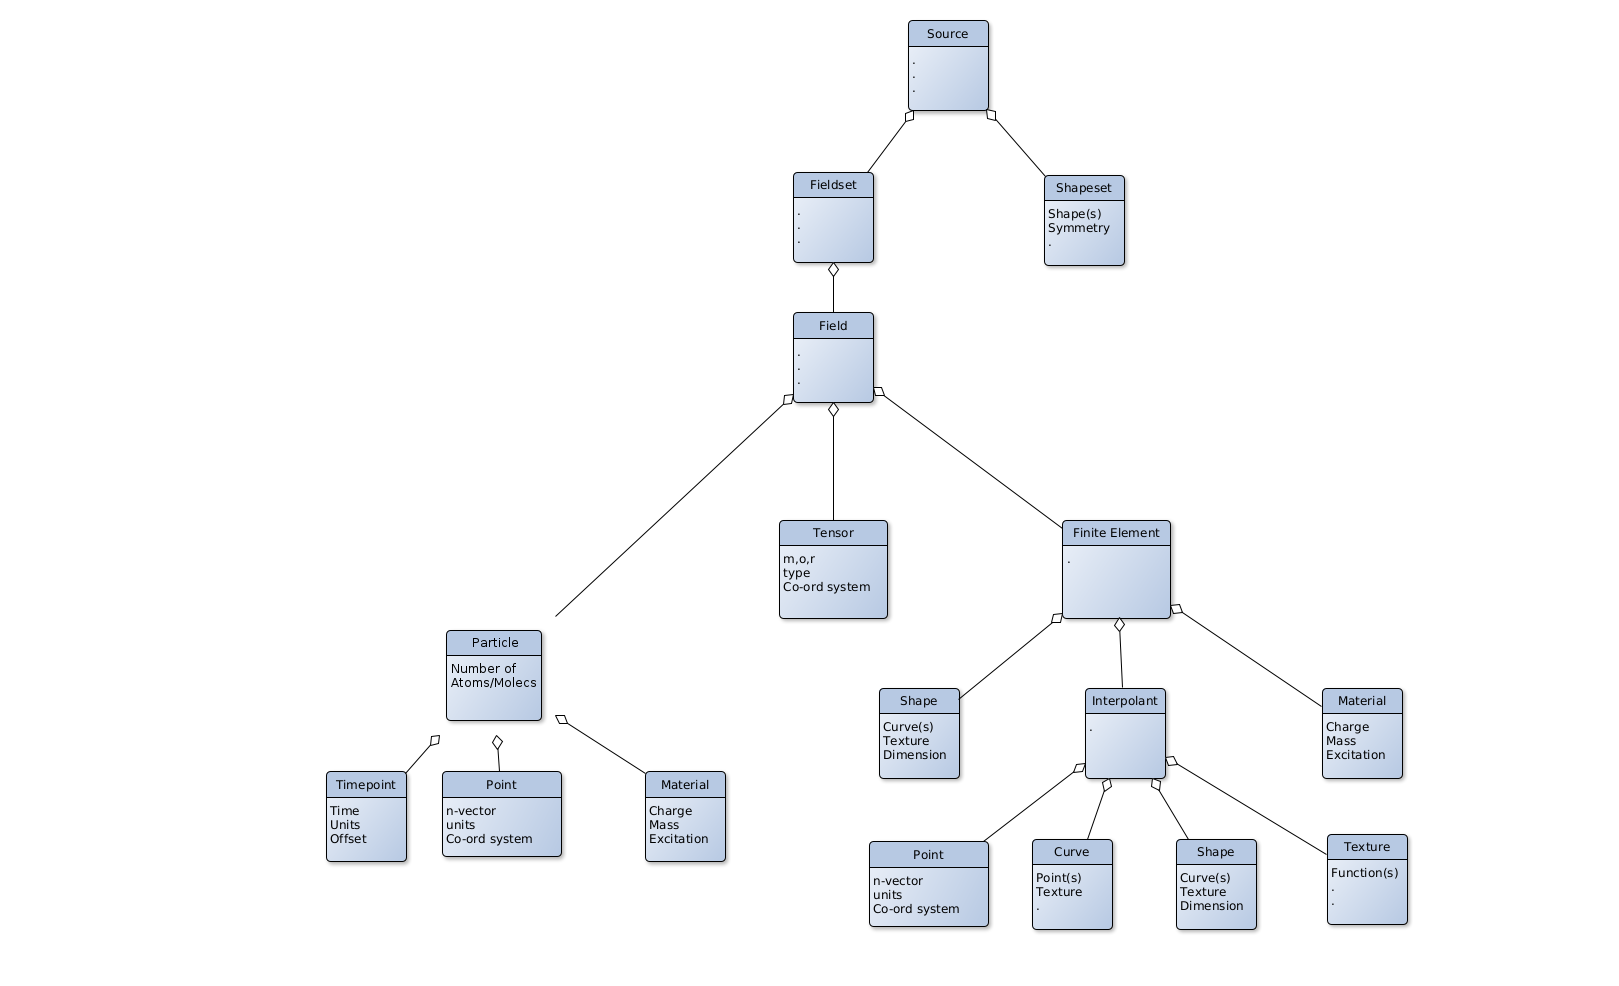
\includegraphics[width=0.7\textwidth]{./pics/aggregates.png}}
\caption{Aggregation of base classes to form a class `Source'.
\label{fig:aggregates}}
\end{figure}
\begin{itemize}
\item
  Particle : parts are location, velocity, material;\\
  Attributes of particle weight
\item
  Interpolant : parts are points, curves, shapes, textures, or
  timepoints, textures
\item
  Diagnostic : parts are DSL input instructions \textbf{Diagnostic
  Processing}, fieldset
\item
  FE (Finite element) : parts are shape, interpolant, material
\item
  Field : parts are tensors and finite elements, or particles;\\
  many make fieldset
\item
  Fieldset : parts are fields
\item
  DE (Differential equation) : parts are operators (DSL input), IC, BC
  and source
\item
  Model : parts are \textbf{Solution of DEs}
\item
  Source : parts are shapeset, fieldset. See \Fig{aggregates}.
\item
  Matexture : parts are materials, textures
\item
  Body : parts are shapeset, matexture
\item
  BC (Boundary Condition) : parts are surface, material, texture
\item
  GEOQ (Geometry plus B-Equil) : parts are shapeset, field
\end{itemize}

\subsection{Simple inherits}\label{sec:simple_inherits}

\begin{itemize}
\item
  HDS (Hierarchical Data Structure) : multi-octree, is a shapeset
\item
  Trajectory : particle position as time varies, is a curve
\item
  IC (Initial Condition) : is a fieldset
\end{itemize}

\subsection{Solution of Differential Equations}\label{sec:solution_of_des}

Use in part ABSTRACT CALCULUS and PUPPETEER patterns (cf.~GoF FACADE)
from Rouson et al. \cite{rousonxiaxu}, see \Sec{desi_patt}.

\subsection{Diagnostic Processing}\label{sec:diagnostic_processing}

\begin{enumerate}
\def\labelenumi{\arabic{enumi}.}
\item
  Read configuration file
\item
  Determine whether any diagnostic needed at present physical time
\item
  Select input fieldset
\item
  Select diagnostic type, use in part ABSTRACT CALCULUS from Rouson et
  al. \cite{rousonxiaxu}

  \begin{itemize}
  \item
    Initial logs

    \begin{itemize}
    \item
      UUID
    \item
      Key input data
    \item
      Key properties, eg. LCFS
    \end{itemize}
  \item
    Combinations of

    \begin{itemize}
    \item
      Field / quadratic field (eg. power, flux quantity) / general
      formula
    \item
      Point, line integral, surface integral, volume integral
    \end{itemize}
  \item
    Mass/charge, momentum/current and power balances
  \item
    Turbulence statistics - cross-correlations, spectra (not particle,
    ray)
  \item
    Difference between solutions/experiment (RMS as `skill') (not
    particle, ray)
  \item
    See ``emergent physics as diagnostic'' in imas\_objects.tex
  \end{itemize}
\item
  Calculate output fieldset
\item
  Set output format
\item
  Output fieldset to disk, screen
\end{enumerate}

\subsection{Orchestration}\label{sec:orchestration}

\begin{enumerate}
\def\labelenumi{\arabic{enumi}.}
\item
  UQ Framework VECMAtk and Fab\nep
\item
  GUI
\item
  CLI
\item
  Possible restart (OLYMPUS logic, Fig.1 of \cite{y2re312})
\item
  \textbf{Initialise} from functions.md
\item
  \textbf{Solution} from functions.md
\end{enumerate}

\clearpage
\newsection{Execution sequence}{sec:DDF_sequence}
\subsection{Preprocessing and
components}\label{preprocessing-and-components}

\begin{itemize}
\item
  Convert equilibrium B-field to standard format (ie. a standard
  resembling EQDSK)
\item
  Convert n-D geometry (NURBS) to opensource format
\end{itemize}

\subsection{Initialise}\label{sec:initialise}

\begin{itemize}
\item
  Convert n-D mesh to readable format
\item
  Assign boundary conditions to mesh (finite element by finite element)
\item
  Validate inputs (eg. Python Cerberus)
\item
  Initialise fields, possibly exploiting toroidal symmetry

  \begin{itemize}
  \item
    using sources, calculate with possibly simplified dynamics
  \item
    semi-analytically (Gaussian in vel. space)
  \item
    random perturbations
  \item
    from disk file
  \item
    from previous calculation
  \item
    apply operators to field (eg.\ EQDSK data \(\rightarrow\) B-Equil)
  \item
    combine vacuum field and B-Equil
  \end{itemize}
\item
  Calculate LCFS
\item
  Normalise field
\item
  Distribute mesh across processors
\item
  Distribute particles across processors
\end{itemize}

\subsection{Solution}\label{sec:solution}

\begin{itemize}
\item
  Extra outer loop over parameters (UQ Framework)
\item
  Outer loop over time
\item
  Inner loop over solver

  \begin{itemize}
  \item
    loop over particles
  \item
    loop over rays
  \end{itemize}
\item
  More deeply nested iteration
\item
  Convergence test
\item
  Rouletting particles
\item
  Particle collision

  \begin{itemize}
  \item
    with geometry
  \item
    with other particle
  \end{itemize}
\item
  Adaptive meshing
\item
  Construct surrogates (UQ Framework)

  \begin{itemize}
  \item
    Reduce in n-D (\(n \rightarrow n-1\))
  \item
    Combine particles
  \item
    Replace particles by FE
  \item
    Smoothing
  \item
    Gyro-averaging
  \item
    Sparse models for Data Assimilation (via SINDy)
  \item
    Gaussian Process
  \item
    Polynomial Chaos Expansion
  \item
    Active Subspaces
  \item
    PGD
  \end{itemize}
\item
  Connect surrogates (UQ Framework)
\end{itemize}

\subsection{Assortment}\label{sec:assortment}

\begin{itemize}
\item
  Calculate HDS from Field geometry data
\item
  Intersect triangle with cuboid
\item
  Calculate surface normal and tangents, curvatures
\item
  Calculate curve tangent and normals, torsion, curvature
\item
  Calculate volumes
\item
  Locate point in field element geometry data
\item
  Select algorithms
\item
  Label with physical units, array dimensions, transformations
\item
  Increase in n-D (\(n \rightarrow n+1\))
\item
  Replace FE by particles
\item
  Evaluate FE representation at set of points
\end{itemize}

\subsection{Diagnostics}\label{sec:diagnostics}

\begin{itemize}
\item
  Calculate terms in power balance
\end{itemize}

\subsection{Utilities}\label{sec:utilities}

\begin{itemize}
\item
  Format conversion
\item
  sorting
\end{itemize}

\subsection{Mathematical library operations}\label{sec:mathematical-library-operations}

\begin{itemize}
\item
  FFT (FFTW package)
\item
  linear algebra
\item
  quadrature
\item
  optimisation
\item
  geometry transformations on point and tensor
\item
  Interpolation STRATEGY to select among

  \begin{itemize}
  \item
    splines (2-D, 3-D)

    \begin{itemize}
    \item
      regular (de Boor)
    \item
      local
    \item
      Weiland
    \end{itemize}
  \item
    Fourier interpolation
  \item
    rational interpolation
  \item
    Lagrange interpolation (after Trefethen)
  \end{itemize}
\end{itemize}

\newsection{Design patterns}{sec:desi_patt}
The design patterns likely to be most relevant to \nep \ are described
in refs~\cite{y2re332,y2re333}.

The PUPPETEER pattern appears to be
exclusive to the works of Rouson~et~al, hence is described further here.
It is directed towards the calculation of the Jacobian of multi-component
systems typically needed for Newton-Raphson type solution of update equations.
The idea is that the puppeteer need only know which blocks of the Jacobian
matrix are nonzero, although the puppets need to be capable of forming derivatives
with respect to all state variables.
\begin{figure}
\centerline{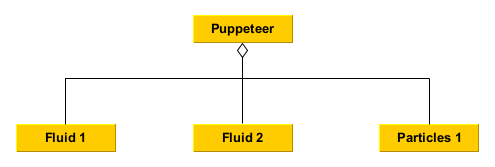
\includegraphics[width=0.95\textwidth]{./pics/puppeteer_wab.png}}
\caption{
PUPPETEER pattern. Each puppet (`Fluid~1', `Fluid~2', `Particles~1') may include terms  involving 
the other puppets. For example, suppose the puppet for `Fluid~1' has terms involving also `Particles~1'
variables (but not `Fluid~2'), then the puppeteer can request derivatives of the puppet's terms both
with respect to `Fluid~1' and `Particles~1' variables, but knows not to ask for derivatives with respect
to `Fluid~2' variables.
\label{fig:puppeteer_wab}}
\end{figure}

